\documentclass[a4paper]{article}

\usepackage{graphicx}
\usepackage[english]{babel}
\usepackage[utf8x]{inputenc}
\usepackage[T1]{fontenc}
\usepackage{sectsty}
\usepackage{pdfpages}
\usepackage[section]{placeins}
\usepackage{float}% If comment this, figure moves to Page 2
\usepackage{listings}
\usepackage{caption}
\usepackage{subcaption}

\setlength\parindent{0pt}
%\setlength{\parskip}{\baselineskip}

%\sectionfont{\fontsize{12}{15}\selectfont}

\begin{document}

\title{Software Architecture Process And Management}
\date{}
\author{Computer Science 4th Year, Created By Monkeys}
\maketitle
\newpage

\tableofcontents
\newpage


\section{Introduction}
\subsection{Learning Outcomes of the course}
\begin{itemize}
\item Integrate knowledge of software architecture to capture \textbf{quality attribute} requirements for a system, \textbf{evaluate proposed architectures} and create options for \textbf{improvement}.

\item Analyse and justify complex \textbf{trade-off decisions} between \textbf{competing software architectures}.

\item Evaluate the \textbf{strengths} and \textbf{weaknesses} of software architecture in support of particular approaches to \textbf{design}, \textbf{process} and \textbf{management} for a particular system and make \textbf{recommendations} on the \textbf{choice of process} for that system.

\item Working in a group to \textbf{critically reflect} on aspects of the \textbf{software architecture literature} and practice to create a resource that support their learning in software architecture.
\end{itemize}

\subsection{What is Success for a Large Project?}
A large project will be considered successful if:
\begin{itemize}
\item The software is delivered on schedule
\item Development costs are within budget
\item The software meets the needs of users
\end{itemize}

\subsection{Software Architecture}

\underline{\textbf{Software Architecture Definitions}}
\begin{enumerate}
\item The software architecture of a system is the \textbf{set of structures} needed to reason about the system, which comprise software elements, relations among them and properties of both. (Bass, Clements, Kazman 2013)
\item A software system's architecture is the set of \textbf{principal design decisions} about the system (R.N Talyor et al)\\
\end{enumerate}

\underline{\textbf{Architecture is a collection of structures}}\\
We observe three frequently types of structure:
\begin{enumerate}
\item \textbf{Modular Structure}: static structure that focuses on how the functionality is divided up, structured, and assigned to development and implementation teams.
\item \textbf{Component and Connector structure}: runtime structures that focus on how components interact.
\item \textbf{Allocation structures}: mapping to organizational, development, installation, execution environments.\\
\end{enumerate}

\underline{\textbf{Architecture is an Abstraction}}\\

Architecture is used to \textbf{suppress} detail that is unimportant for the reasoning we are doing. In particular it \textbf{abstracts away} from the private details of \textbf{implementation details} of specific methods.\\

** All systems have architectures (even if people have forgotten them) **\\

Complicated systems are embedded in organisation and we can often see architecture through practice:
\begin{itemize}
\item \textit{How is the system developed?} -> This will often provide \textbf{clues to structures}.
\item \textit{How is the maintenance, evolution, issue reporting dealt with?} -> This will often help with \textbf{modularity}.
\item \textit{What are the failure characteristics of the system in operation?} -> This will often suggest \textbf{component and connector structure}.
\end{itemize}


\subsection{Case Study: General Practice Extraction System}

"The General Practice Extraction Service (GPES)" is an IT system designed to allow NHS organizations to extract data from \textbf{all} GP practice computers. \textit{This is because different GP's have different contracts and therefore use different software to save patient data.}\\

Basic idea is to create an API to query every system from all different software's created for different GP's. This will allow generic extraction of \textbf{patient data} regardless of their GP.

% IMAGE: GPES Customers
\begin{figure}[H]
\centering
\begin{subfigure}{1\textwidth}
  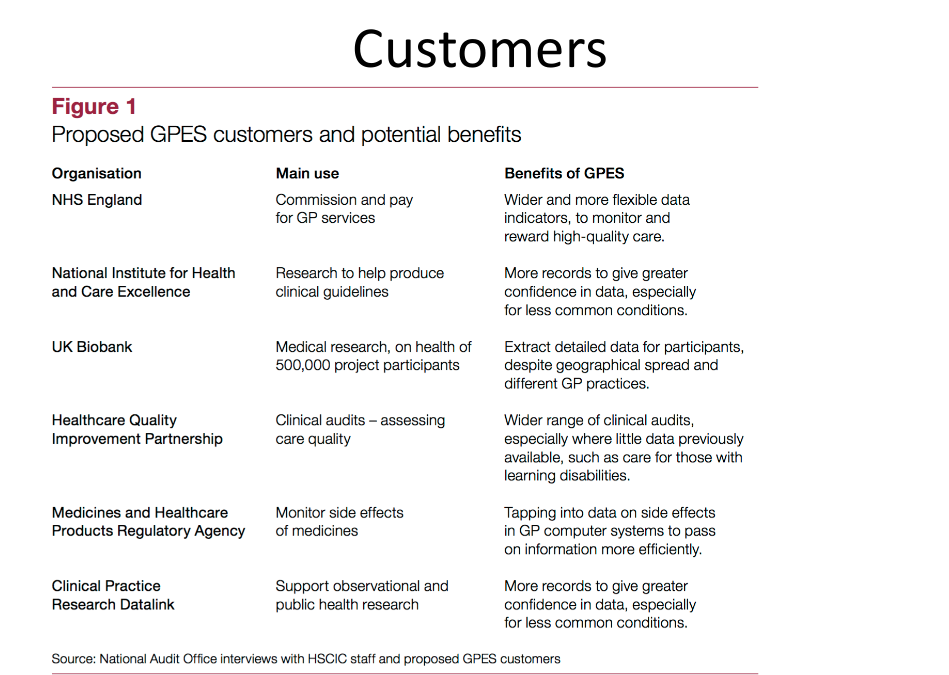
\includegraphics[width=1\linewidth]
  {images/1-customers.png}
\end{subfigure}
%\caption{-}
\end{figure}


% IMAGE: GPES Structure
\begin{figure}[H]
\centering
\begin{subfigure}{1\textwidth}
  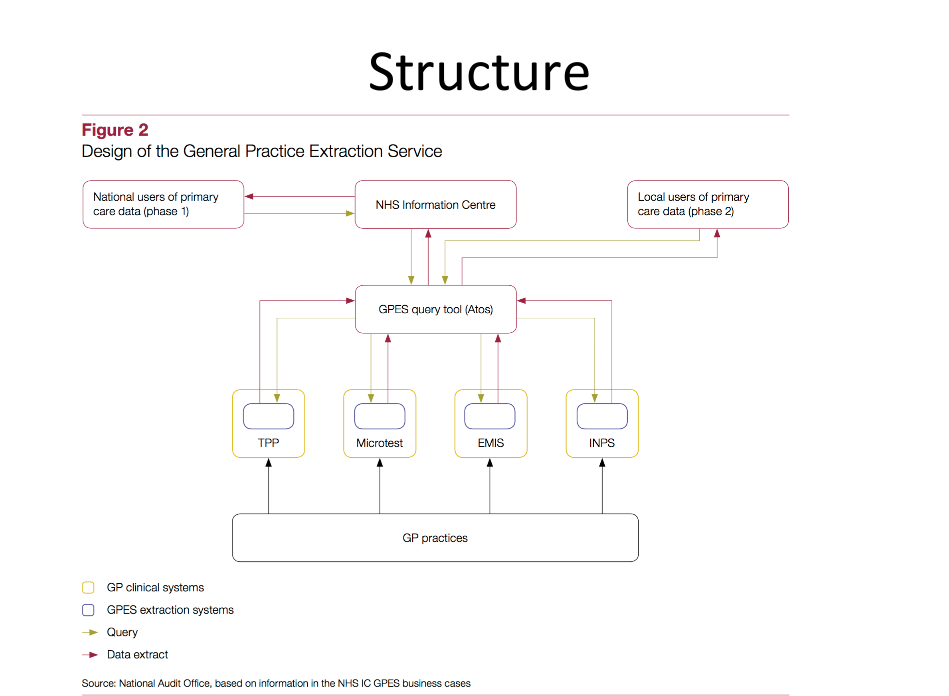
\includegraphics[width=1\linewidth]
  {images/1-structure.png}
\end{subfigure}
%\caption{-}
\end{figure}

% IMAGE: GPES Timeline
\begin{figure}[H]
\centering
\begin{subfigure}{1\textwidth}
  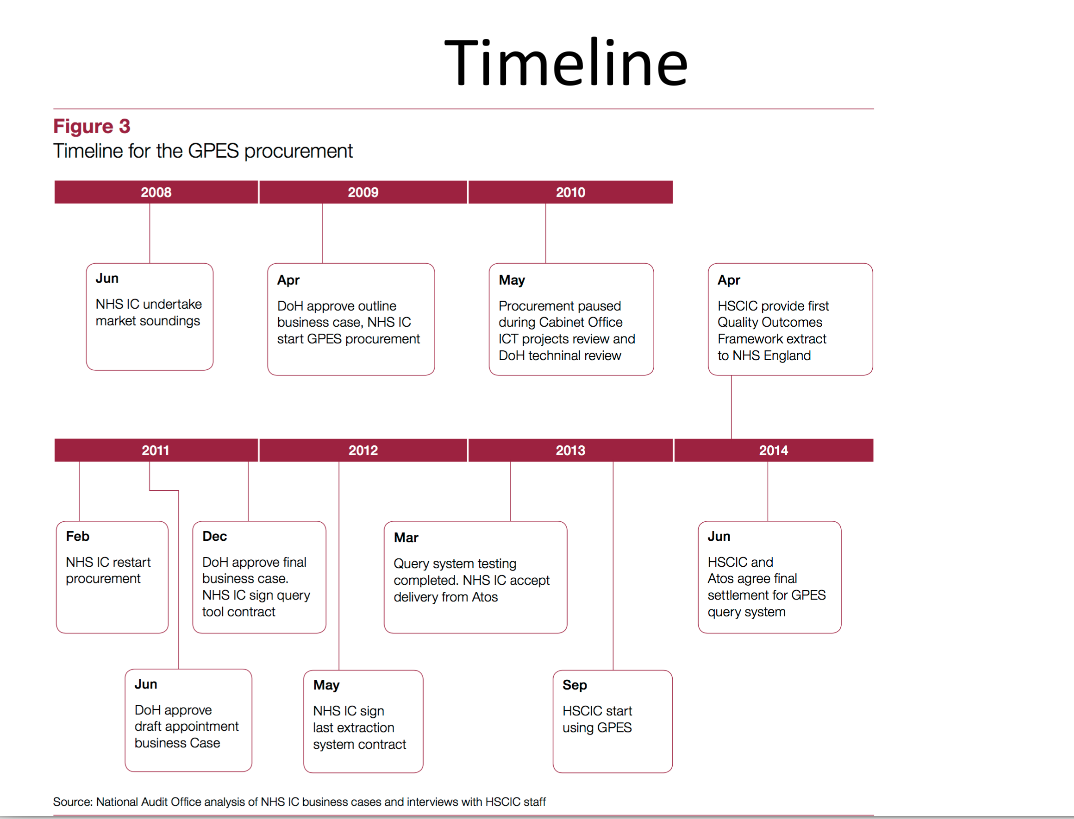
\includegraphics[width=1\linewidth]
  {images/1-timeline.png}
\end{subfigure}
%\caption{-}
\end{figure}


\underline{\textbf{National Audit office Conclusion of the GPES Project}}
\begin{itemize}
\item The project has been significantly delayed and many customers have yet to receive data.
\item Mistakes in the original procurement and contract management contributed to the losses of public funds. This occurred through asset write-off's and settlements with suppliers
\item Only \textbf{one} customer, \textit{NHS England} has so far received data from GPES.\\
\end{itemize}

Originally the business plan for GPES said the service would start in \textbf{2009-2010}. It actually took until \textbf{2014} for the first extraction to take place. The total expected loss for the GPES project rose from \textbf{£14 million} to \textbf{£40 million} during the \textit{planning} and \textit{procurement stage}.\\

\underline{\textbf{Data Extract Issues}}
\begin{itemize}
\item First GP system suppliers were asked to fulfil a common query language for the extraction process (this was not in their interest as it would cost them alot to makes these changes to their current systems and thus pretty much refused to do so).
\item This requirement then changed to each GP system supplier creating their own logical 'business rules' which would be used to extract the data. (Different for each supplier, one API to query each supplier to extract data)
\item NHS IC's using a non-competitive procurement approach, in-addition to the changes in design both contributed to the restrictive process for \textit{extracts}.
\item HSCIC (the successor of the NHS IC) has continued to use the GPSOC framework to require data sharing between NHS systems. \textit{The new framework (2014) states that the principal clinical system suppliers must provide an interface method for third-party system uses.}

\item \textbf{HSCIC cannot do wide range nor scale of data extracts. Due to the design of the GPES system and the restrictions in the supplier contracts. (Over 100 different extracts have been requested) HSCIC estimate that they will only be able to design 24 new extracts in 2015-16}\\
\end{itemize}

% IMAGE: GPES Issues
\begin{figure}[H]
\centering
\begin{subfigure}{1\textwidth}
  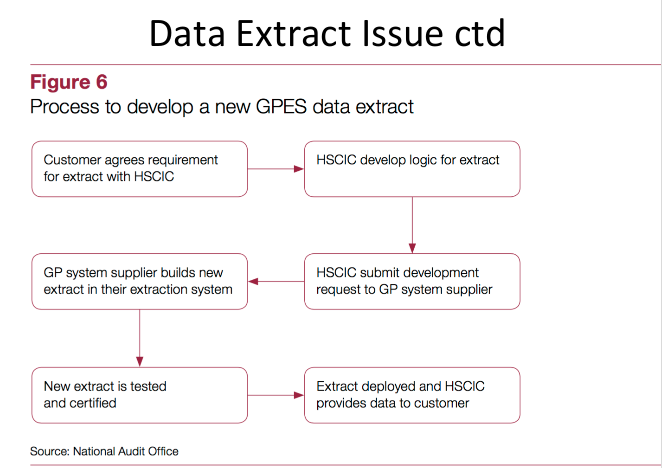
\includegraphics[width=1\linewidth]
  {images/1-issues.png}
\end{subfigure}
%\caption{-}
\end{figure}

% IMAGE: GPES Issues Concluded
\begin{figure}[H]
\centering
\begin{subfigure}{1\textwidth}
  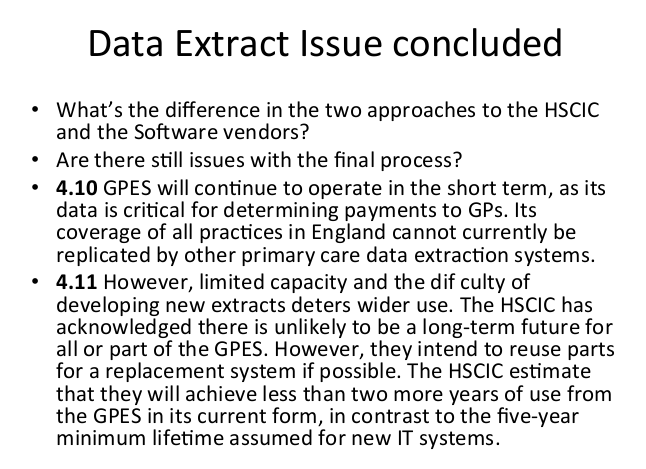
\includegraphics[width=1\linewidth]
  {images/1-issues-concluded.png}
\end{subfigure}
%\caption{-}
\end{figure}
\newpage

\section{Basic Concepts of Architectures}
\subsection{What is good architecture?}
The architecture is appropriate for the \textbf{context of use}. E.g. 3-tier e-commerce architecture is not appropriate for a avionics project.\\

Guidance on 'good architecture' focuses on:
\begin{itemize}
\item \textbf{Process}
\item \textbf{Structure}\\
\end{itemize}



Software architecture should capture the \textbf{principal design} decisions about the system. The \textbf{Blueprint} for software architecture focuses on:
\begin{itemize}
\item Structure
\item Component behaviour
\item Component interaction and how that influences \textbf{Quality Attributes} of the \textit{systems}.\\
\end{itemize}

\subsection{Process}
Architect teams are often small and \textbf{maintains the integrity} of the architecture. The architecture is \textit{justified} in relation to a \textbf{prioritized list of quality attributes} that need to be managed. \textbf{Stakeholders interests} are documented and are used to build the type of architecture that will reflect them.\\

Architecture is often evaluated in terms of \textit{how well it delivers the quality attributes}. Software architectures are often chosen to allow \textbf{incremental implementation}. (I.e Low coupling, high cohesion)

- Definitions for coupling and cohesion!

\subsection{Structure}

The structure of architecture will differ depending on the requirements of the software, often the following are utilised:
\begin{itemize}
\item \textbf{Modularity} $\rightarrow$ Hides information, separates concerns, allows good robust interfaces that are unlikely to change
\item Well known \textbf{patterns and tactics} are often implemented
\item Architecture built to NOT depend on \textbf{particular versions of tools}, or \textbf{special features} \textit{unless its essential!}
\item Modules \textit{producing} data should be \textbf{separate} from those \textit{consuming} data
\item Usually a complex mapping between \textbf{modules} \textit{(static structure)} and \textbf{components} \textit{(dynamic structure)}
\item MINIMISE the number of ways of \textbf{interaction between components}
\item The architecture should clearly \textbf{identify resource contention issues} and deal with them. (E.g. network capacity, minimise network throughput using different techniques [EXC])\\
\end{itemize}

\underline{\textbf{Prescriptive vs Descriptive Structures}}\\
\textbf{Prescriptive} structure is what we use to model the system before it is built. It is the aim the architect has while generating the blueprint \textit{(UMLAsBlueprint, forward engineering)}, however it is often to \textit{tidy} and unrealistic to be able to model the architecture of a system.\\

\textbf{Descriptive} structure is usually made after the system has been created. It is used to describe the entire system, how the \textbf{components} interact, the responsibilities of each \textbf{module} \textit{(usually extremely messy)} etc ...

\subsection{The Importance of Architecture}
Software Architecture has several uses:
\begin{enumerate}
\item Enables us to manage the \textbf{key attributes} of a system
\item Allows reasoning about and managing \textbf{change}
\item Allows predictions of \textbf{key quality attributes}
\item Allows \textbf{improved communication} between stakeholders
\item Defines \textbf{constraints} on the software's implementation
\item Provides the basis for \textbf{evolutionary prototyping}
\item Is the key artefact for reasoning about \textbf{cost} and \textbf{scheduling}
\item Focuses on the assembly of \textbf{components} rather than the \textbf{creation/implementation} of components\\
\end{enumerate}

Other uses are:
\begin{itemize}
\item \textit{Reflects the structure of an organisation}
\item \textit{Can be used as the transferable, reusable model at the heard of a product line}
\item \textit{Restricts design alternative and channels developer effort in a coordinated way}
\item \textit{Provides the basis for training new team members}
\end{itemize}

\subsection{Managing Attributes and Change}
It is a fact that the majority of software projects will undergo requirements change. This may also change \textbf{key quality attributes} of the system. The idea is to use architecture that will minimise the change to the \textit{architecture} and allow the system to be \textbf{modifiable} utilising the same abstract \textbf{architectural} ideas.\\

Managing change can be reasoned about on three levels:
\begin{enumerate}
\item Inside an element \textit{[cheapest]}
\item Between elements maintaining the architecture \textit{[can be costly]}
\item Requiring architecture change (we wish to avoid this as much as possible) \textit{[most expensive change]}
\end{enumerate}

\subsection{Prediction of Attributes}
We can attempt to predict the \textbf{key quality attributes} of the system based on \textit{requirements} and possible (logical) \textit{system extensions} in the future. Planning for these changes will minimise need for architectural change, which in turn will \textbf{reduce the cost} in future work.\\

\textbf{** Models should be able to be built based on the predictions of the attributes and requirements **}


\subsection{Communication Between Stakeholders}
A well documented architecture allows \textbf{improved communication} between stakeholders. Some examples of how the documented architecture can help with communication are the following:
\begin{itemize}
\item User has particular requirements in terms of user experience
\item Customer needs to know about schedule, budget and meeting regulations in their market
\item Project manager needs to know the dependences in terms of the modules and components
\end{itemize}
\underline{\textit{These might be accommodated by different views of the system that are consistent}}

\subsection{Early Design and Constraints}
Early design carries the \textit{most fundamental} design decisions, e.g:
\begin{itemize}
\item What the \textbf{key quality attributes} are
\item The \textbf{architecture form/type} that will give the best control over these attributes
\item The characterisation of the behaviour of the architecture elements\\
\end{itemize}

% IMAGE: Constraints
\begin{figure}[H]
\hskip-1.5cm\begin{subfigure}{1.1\textwidth}
  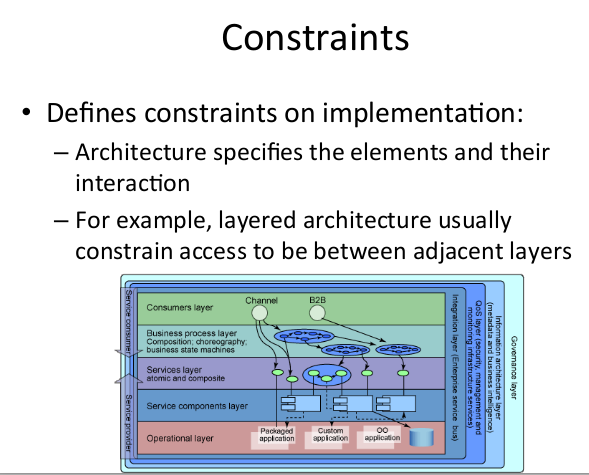
\includegraphics[width=1.2\linewidth]
  {images/2-constraints.png}
\end{subfigure}
%\caption{-}
\end{figure}

\subsection{Evolutionary Prototyping}
\textbf{Evolutionary Prototyping} allows a system to be constantly tested under real conditions as it is being developed. As \textit{bugs} are detected they are fixed and tested in the next prototype. Examples of systems that used \textbf{evolutionary prototyping} are:
\begin{itemize}
\item Plug and Play - early experience of the BASE functionality + extensibility.
\item Real time architectures - early experience with scheduling. \textit{(Worse case execution times guide design and deployment)}
\end{itemize}

\subsection{Cost and Scheduling}
Reasoning about the \textbf{following topics} allows for effect cost and scheduling in a software project:
\begin{itemize}
\item Capturing dependencies
\item Estimation of required efforts for different sections
\item Allocating effort to elements
\item Understanding of how elements influence each other
\item Use architecture to interpret bottom-up estimates from teams working on elements
\end{itemize}

\subsection{Product Line (Model)}
The \textbf{product line} model is a \textit{transferable and reusable} model. \textbf{Elements} are assets that compose to give new \textit{functionality}. The architecture provides the means to \textbf{compose the elements}. A planned approach allows the reuse of architectural elements \textit{(think object inheritance)}.

\subsection{Component Level \& Channelling Development}
At the component level we focus on the \textbf{assembly} of components rather than the \textbf{creation} of them! With well designed elements and architecture we can combine elements from different \textbf{producers} \textit{(provided they conform to a standardized interface)}. This provides the following \textbf{benefits}:
\begin{itemize}
\item Decrease time to market
\item More reliability
\item Lower cost
\item Flexibility \textit{(e.g. using multiple or alternate suppliers for a component)}\\
\end{itemize}

\textbf{Channelling Development} restricts alternatives and channels developer effort in a coordinate way. This provides a defined \textbf{context} for the developer. Well defined \textbf{interfaces} and clear ideas of the \textbf{functionality \& quality attributes} are required!\\

\textbf{** The overall goal is to provide clarity on what is an architectural decision and what is a development decision. **}
\newpage


\section{Context Design}
Software architects and architecture have arisen as systems have grown in: \textit{scale}, \textit{economic importance} and \textit{criticality}. Architecture plays different roles in different contexts. The \textbf{main contexts} are:
\begin{itemize}
\item Technical Context
\item Project Life-cycle Context
\item Business Context
\item Professional Context
\end{itemize}
\subsection{Technical Context}
The \textbf{technical context} is whereby the architecture supports technical activity. For example this could be in \textbf{measuring} a statistic, the \textbf{verification \& validation} process, \textbf{compliance} ...\\

The architecture provides a means for controlling \textbf{quality attributes} of the system. In the \textbf{context of design} activities we try and choose architectures that \textbf{enable the attributes} we care most about. We may find through analysing already \textit{existing systems} that specific architectures inhibit (prevent) particular quality attributes.\\

** Architecture does not often have much to say about the functionality of a system, because they provide containers for functionality. **

\subsubsection{Controlling Quality Attributes}

Usually we care about multiple quality attributes at once. Selecting a type of architecture will allow specific quality attributes to be ensured for when it is deployed to the end user. Examples of \textbf{quality attributes} we might care about for a particular system are:

\begin{table}[H]
\begin{tabular}{|l|p{10cm}|}
\hline
QA & Description\\
\hline
Safety & The safety of a system is whereby we worry about ensuring that the \textbf{system only behaves as is intended} and has no additional behaviour that is unspecified.\\
\hline
Testability & The testability of a system ensures that \textbf{elements are clearly isolated}. That we know the \textbf{expected behaviour of components}. We know the \textbf{relations of modules} to track down faulty code and finally we know how the \textbf{components are intended to integrate together} to give overall behaviour.\\
\hline
Availability & The availability of a system is whereby we worry about ensuring there is a \textbf{system to take over}, in the case the original system fails. \\
\hline
\end{tabular}
\end{table}

Other examples of quality attributes include \textbf{performance}, \textbf{usability}, \textbf{interoperability} ...\\

These examples of quality attributes related to the \textbf{actuator monitoring} system that was described in lectures. As actuators are physical devices they will suffer from \textit{'wear and tear'} and eventually break. In safety critical system (for example cars, aeroplanes) these actuators require monitoring in order to prevent worst-case scenario's when they do break, and have them repaired beforehand.\\

The architecture for the actuator monitoring system will be required to hold at least those three quality attributes:
\begin{enumerate}
\item Availability - To ensure it is always monitoring the actuators
\item Safety - To ensure the monitoring system does not deviate from intended behaviour (no false positives or false negative)
\item Testability - To provide certainty that of the safety and availability is should provide.
\end{enumerate}

% IMAGE: Actuator Monitoring Architecture
\begin{figure}[H]
\centering
\begin{subfigure}{1\textwidth}
  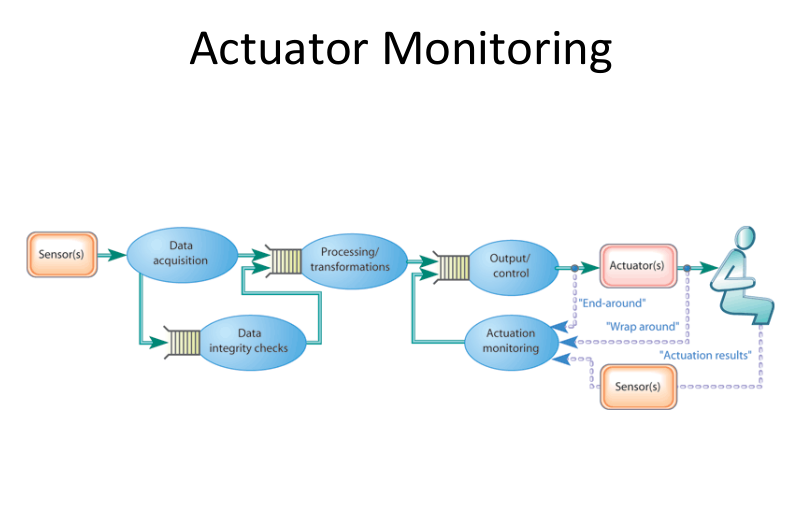
\includegraphics[width=1\linewidth]
  {images/3-actuator-monitoring-architecture.png}
\end{subfigure}
%\caption{-}
\end{figure}


\subsection{Project Life-cycle Context}
The \textbf{project life cycle context} describe how the project will develop over time. The architecture is then created to adopt the life-cycle that is best for a particular project. When creating a project life-cycle the following must be complete \textit{(these are all done best by talking about the architecture)}:
\begin{itemize}
\item Making a business case for the system
\item Understanding the requirements that concern quality attributes
\item Deciding on architecture
\item Documenting architecture
\item Analysing and evaluating architecture
\item Implementing and testing the system based on architecture
\item Ensuring the implementation conforms to the architecture
\end{itemize}

\subsubsection{V-Model}
The \textbf{V-Model} is a development of \textit{waterfall} and explicitly includes architectural design as a stage. It highly focuses on \textbf{requirements based testing} all the way down to the unit level!

% IMAGE: V-Model
\begin{figure}[H]
\hskip-2.5cm\begin{subfigure}{1.2\textwidth}
  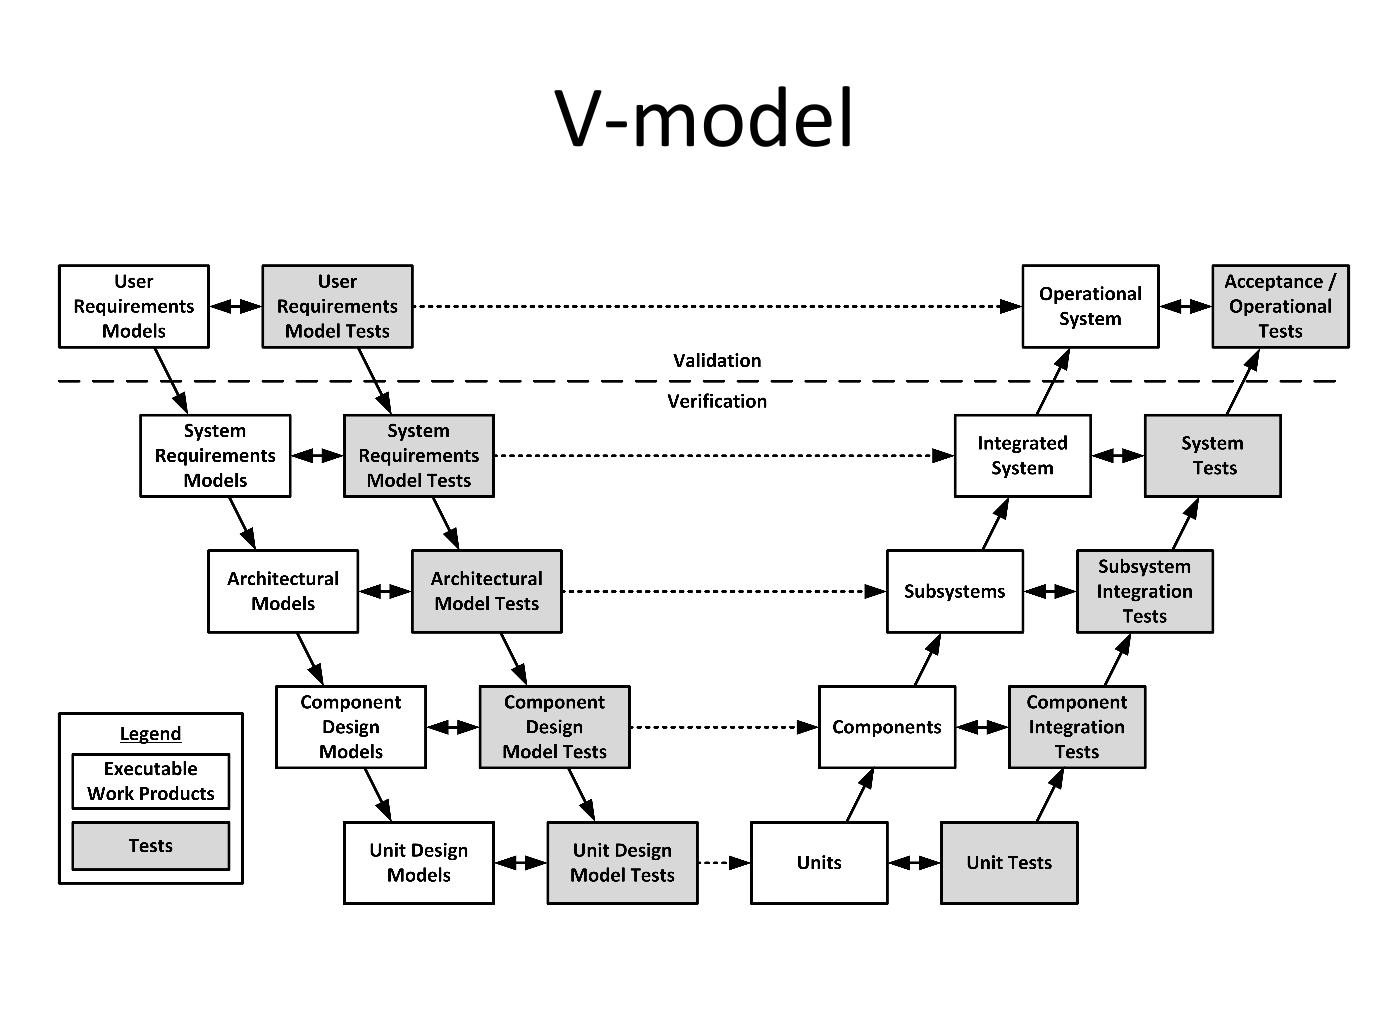
\includegraphics[width=1.2\linewidth]
  {images/3-v-model.png}
\end{subfigure}
%\caption{-}
\end{figure}

\subsubsection{Spiral Model}
The \textbf{(Boehm's spiral model} is a type of \textit{iterative model}. It focuses on project risk management by constantly creating prototypes to be tested all the way through the development life-cycle.

% IMAGE: Spiral
\begin{figure}[H]
\hskip-2.5cm\begin{subfigure}{1.2\textwidth}
  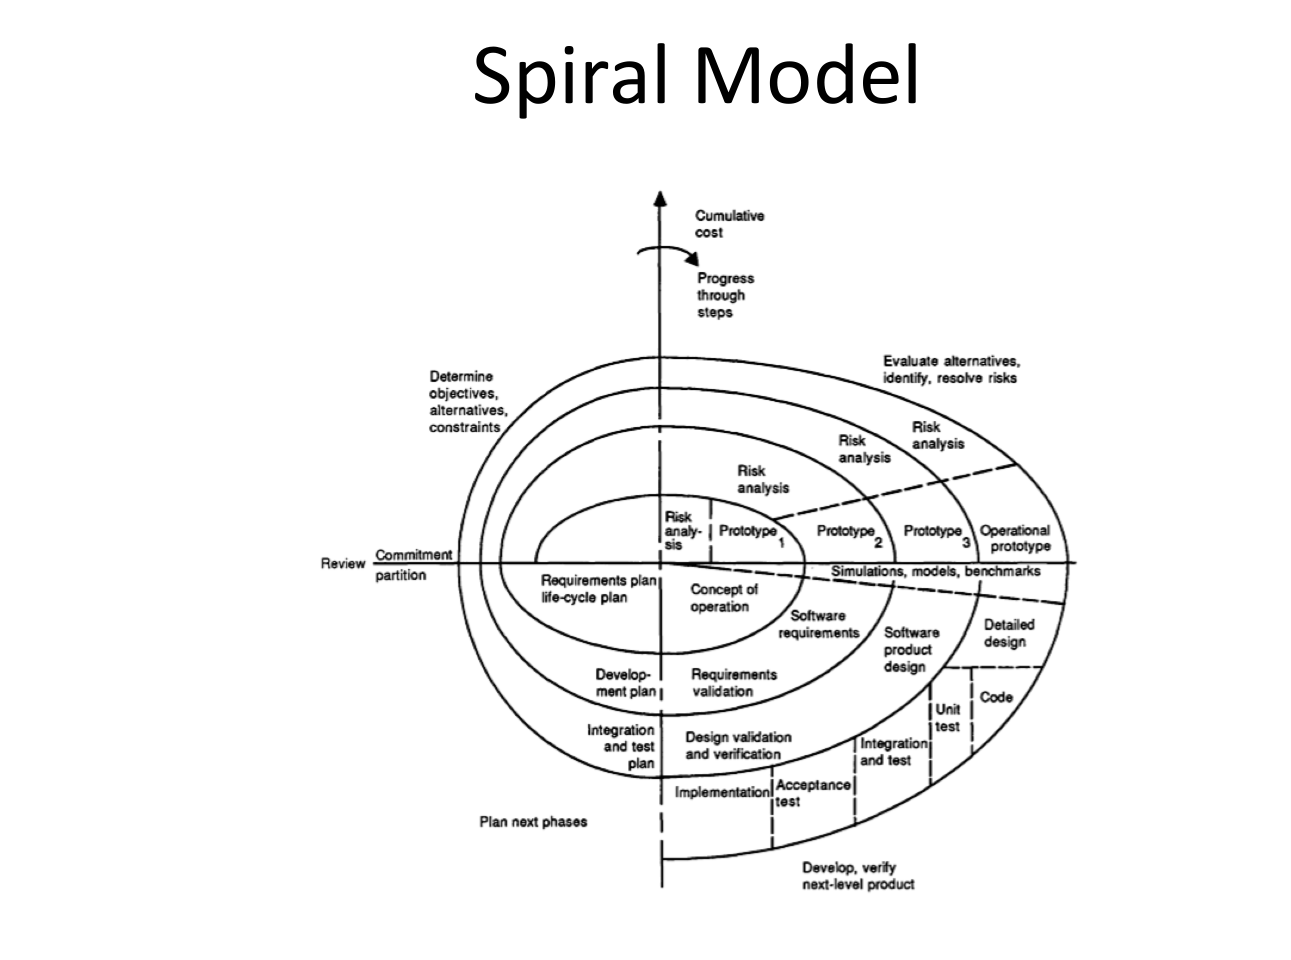
\includegraphics[width=1.2\linewidth]
  {images/3-spiral.png}
\end{subfigure}
%\caption{-}
\end{figure}
\subsubsection{Agile Development}
The \textbf{Agile} development life-cycle is an iterative and incremental method of managing the design and building of a software product. The image below show two different forms of \textbf{agile} development. One with and one without Devops.
% IMAGE: Agile
\begin{figure}[H]
\hskip-2.5cm\begin{subfigure}{1.2\textwidth}
  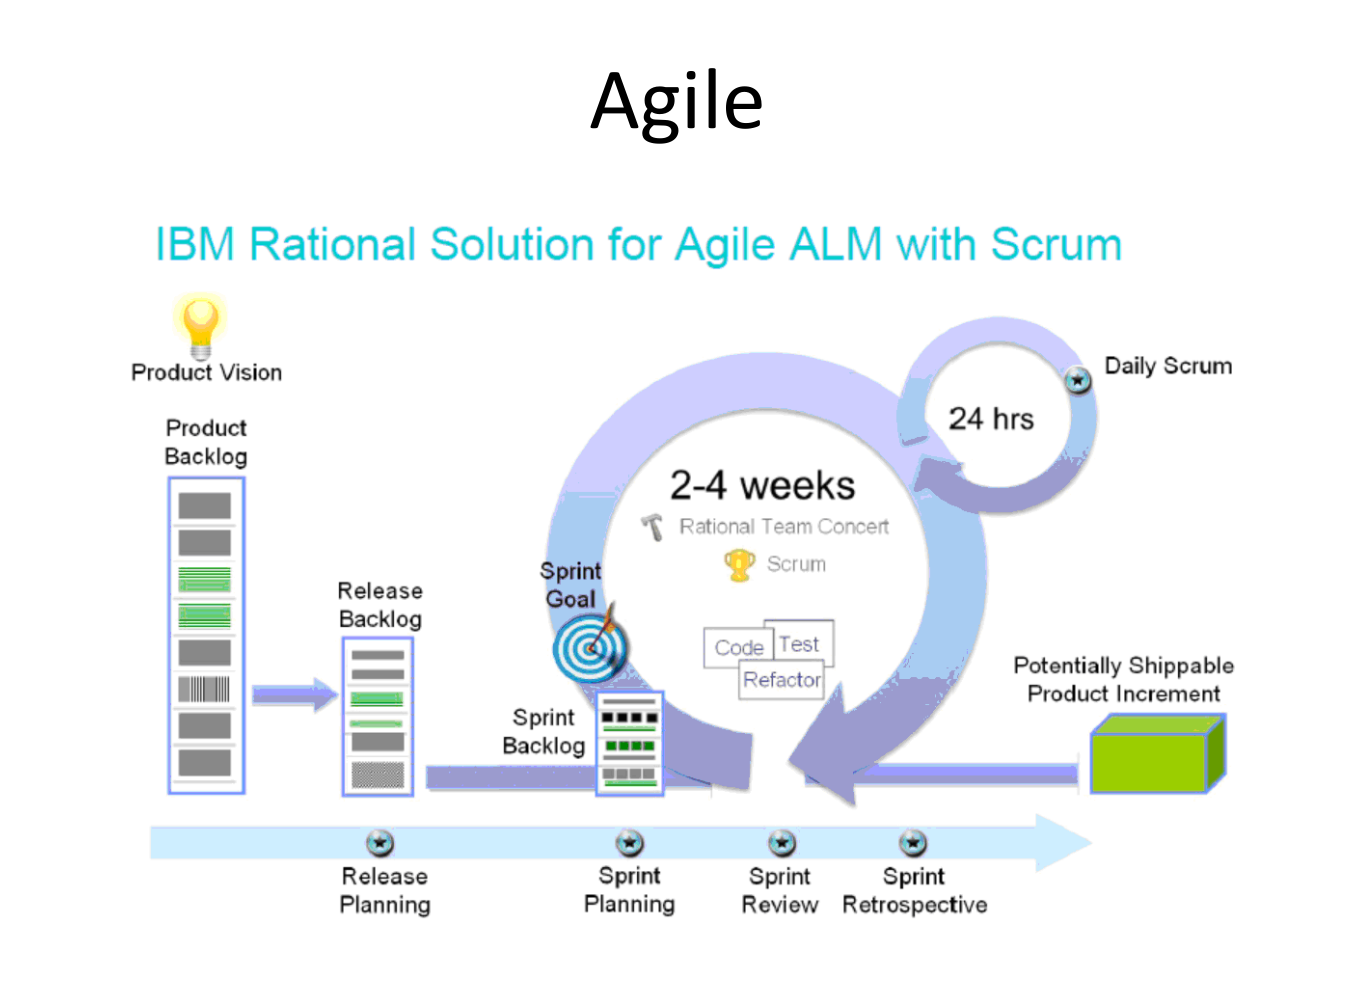
\includegraphics[width=1.2\linewidth]
  {images/3-Agile.png}
\end{subfigure}
%\caption{-}
\end{figure}
\subsubsection{Agile + Devops}
% IMAGE: Agile + Devops
\begin{figure}[H]
\hskip-2.5cm\begin{subfigure}{1.2\textwidth}
  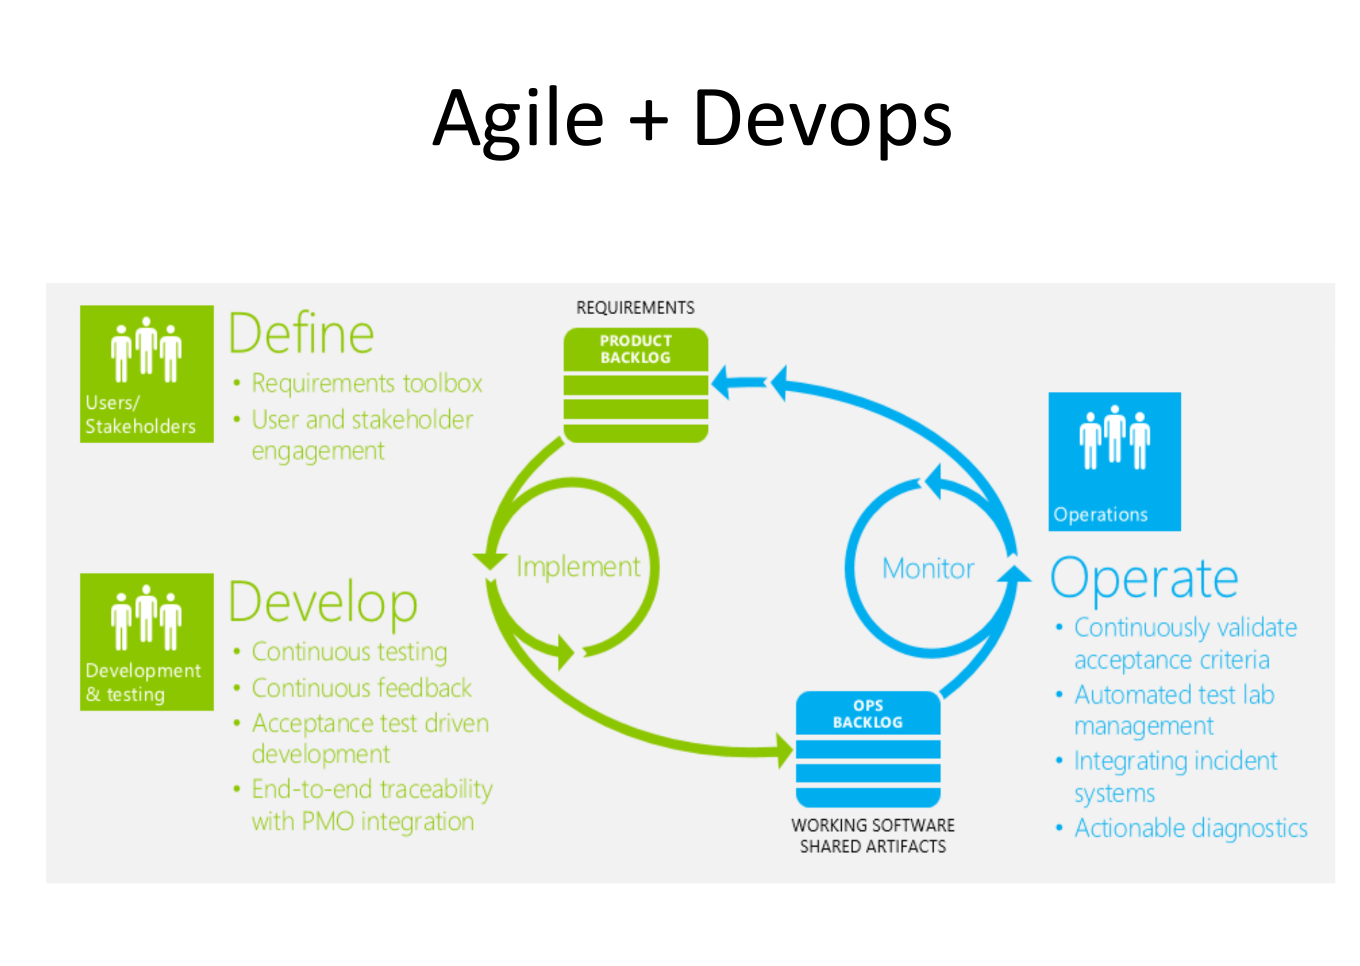
\includegraphics[width=1.2\linewidth]
  {images/3-ADevops.png}
\end{subfigure}
%\caption{-}
\end{figure}
\subsection{Business Context}
The \textbf{business context} is discussed in later lectures. Two aspects we cover are:
\begin{enumerate}
\item How the organisation structure of stakeholders can drive architectural decisions and shapes decisions taking around architecture.
\item How architectural expertise drives the structure of development organisation in terms of their functional units and interrelationships.
\end{enumerate}
\subsection{Professional Context}
The architectural perspective gives you as a professional:
\begin{itemize}
\item A way of describing your expertise
\item Your skills as an architect will be recognised within organisations you work within
\item You can use architecture as a way of describing your past experience
\item You can specialise in particular classes of architecture (e.g. financial architecture)
\end{itemize}
\subsection{Domain-Specific Software Architecture}

\underline{\textbf{Design in the Technical Context}}\\
Design is a mixture of \textbf{creativity} and the use of \textbf{knowledge} that is institutionalised in the context. This takes the form of \textbf{reusable structures}. These reusable structures also influence other aspects of context, helping to shape \textbf{processes, organisations} and \textbf{professions}. We can plot different sorts of \textbf{architectural structures} depending on the degree to which it is \textbf{specific to a domain} and the extent to which it \textbf{influences the system}.\\

% IMAGE:
\begin{figure}[H]
\hskip-2.5cm\begin{subfigure}{1\textwidth}
  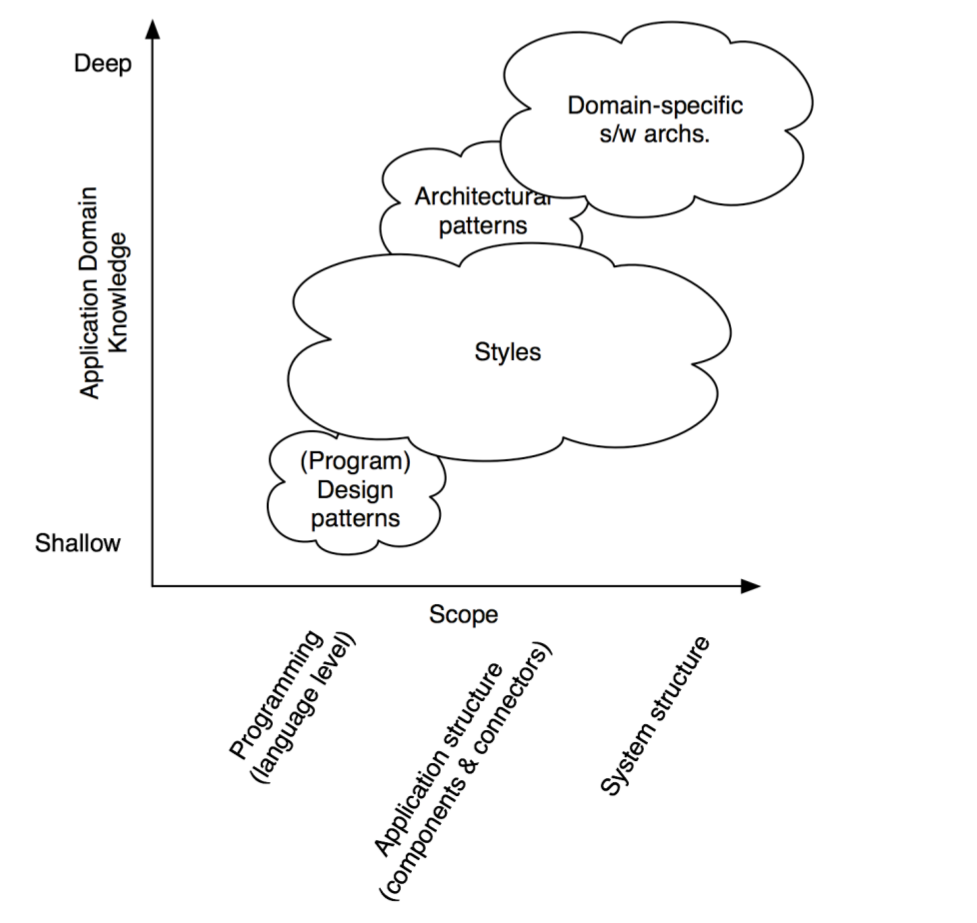
\includegraphics[width=1\linewidth]
  {images/3-graph.png}
\end{subfigure}
%\caption{-}
\end{figure}

\underline{\textbf{Domain Specific Software Architectures}}\\
\textbf{DSSA} is a collection of (pre-decided) \textbf{design decisions}. They capture important aspects of a particular task \textbf{(domain)} They are \textbf{common} across a range of systems in the domain and typically will have some predefined structures depending on the attributes we want to control.\\

These are \textbf{not} general purpose because they incorporate many specific characteristics of the \textbf{domain}. The main benefit is the extent to which \textbf{design knowledge is captured}. There are however problems, over time basic information can be forgotten.\\

** Bridge example given, where key information was forgotten regarding the architecture of suspension bridges (from the 19th century). This results in a bridge collapsing because of wind. **
\subsection{Architectural Patterns}

An architectural pattern is a set of \textbf{architectural design decisions} that are applicable to a \textbf{recurring design problem}, and \textbf{parametrized} to action for different \textbf{software development contexts} in which that problem appears.\\

They are similar to \textbf{DSSA} but capture less of the behaviour and attributes of the system. They are \textbf{more general} because they are intended to abstract a common \textbf{pattern over several domains}.

Three common architectural patterns that are used are listed below:
\begin{enumerate}
\item State Logic Display: Three-Tiered Pattern
\item Model View Controller Pattern
\item Sense Compute Control Pattern\\
\end{enumerate}

\textbf{Contexts shape design.} The \textbf{technical context} identifies features we want to control and \textbf{packages} a range of other properties. Standard architectures (\textit{patterns and domain specific architectures DSSA}) \textbf{package these}. The other context we consider also help to shape the choice of architecture.\\

\textbf{** In design we use pre-decided strcutures and then alter/extend them as and when we need too. **}


% IMAGE:
\begin{figure}[H]
\hskip-2.5cm\begin{subfigure}{1.2\textwidth}
  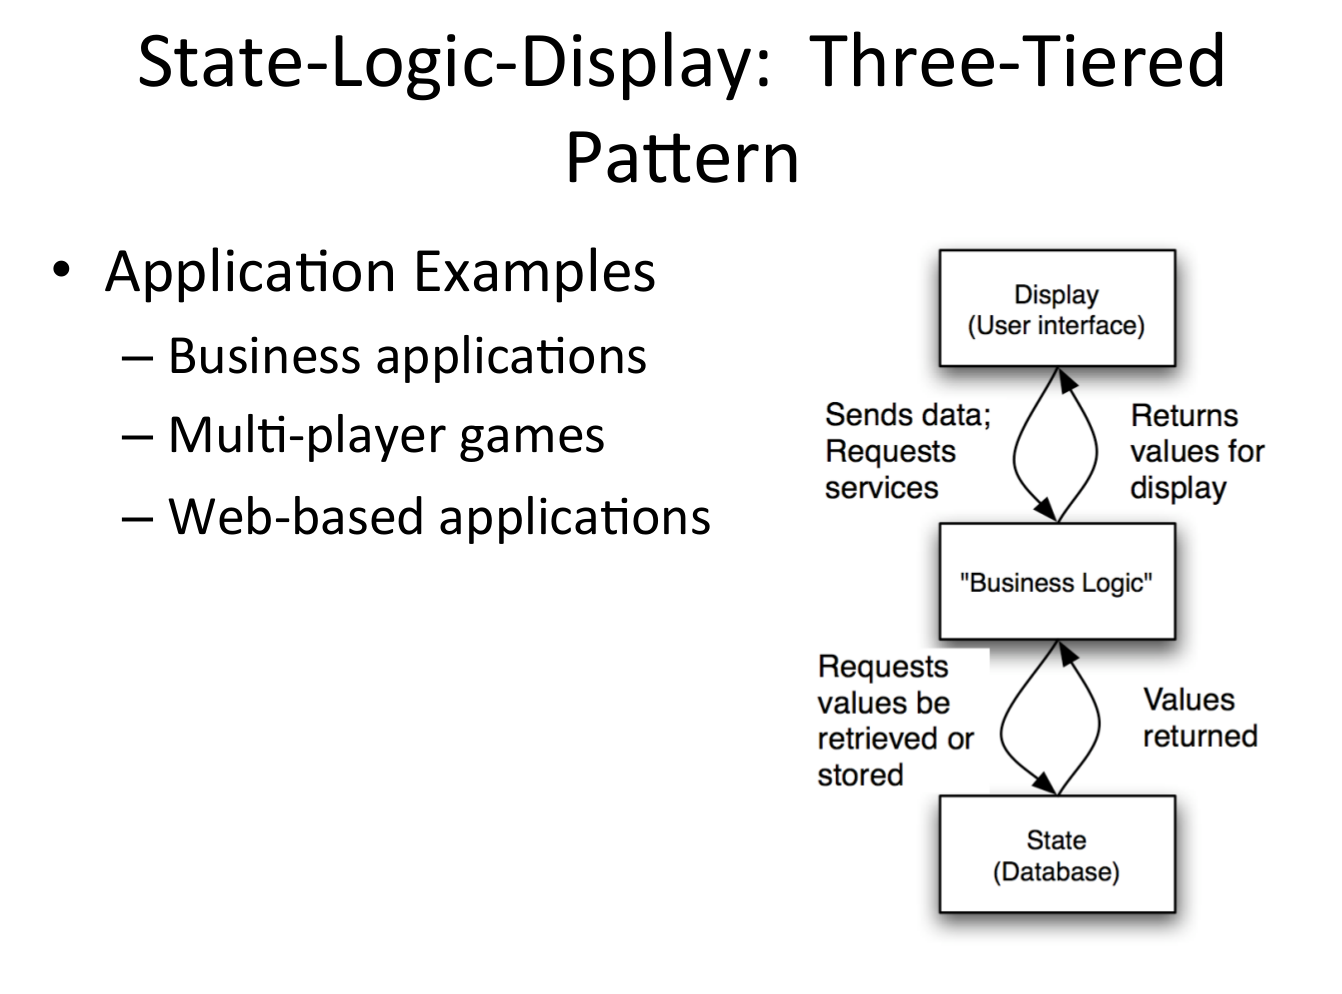
\includegraphics[width=1.2\linewidth]
  {images/3-SLD-pattern}
\end{subfigure}
%\caption{-}
\end{figure}

% IMAGE:
\begin{figure}[H]
\hskip-2.5cm\begin{subfigure}{1.2\textwidth}
  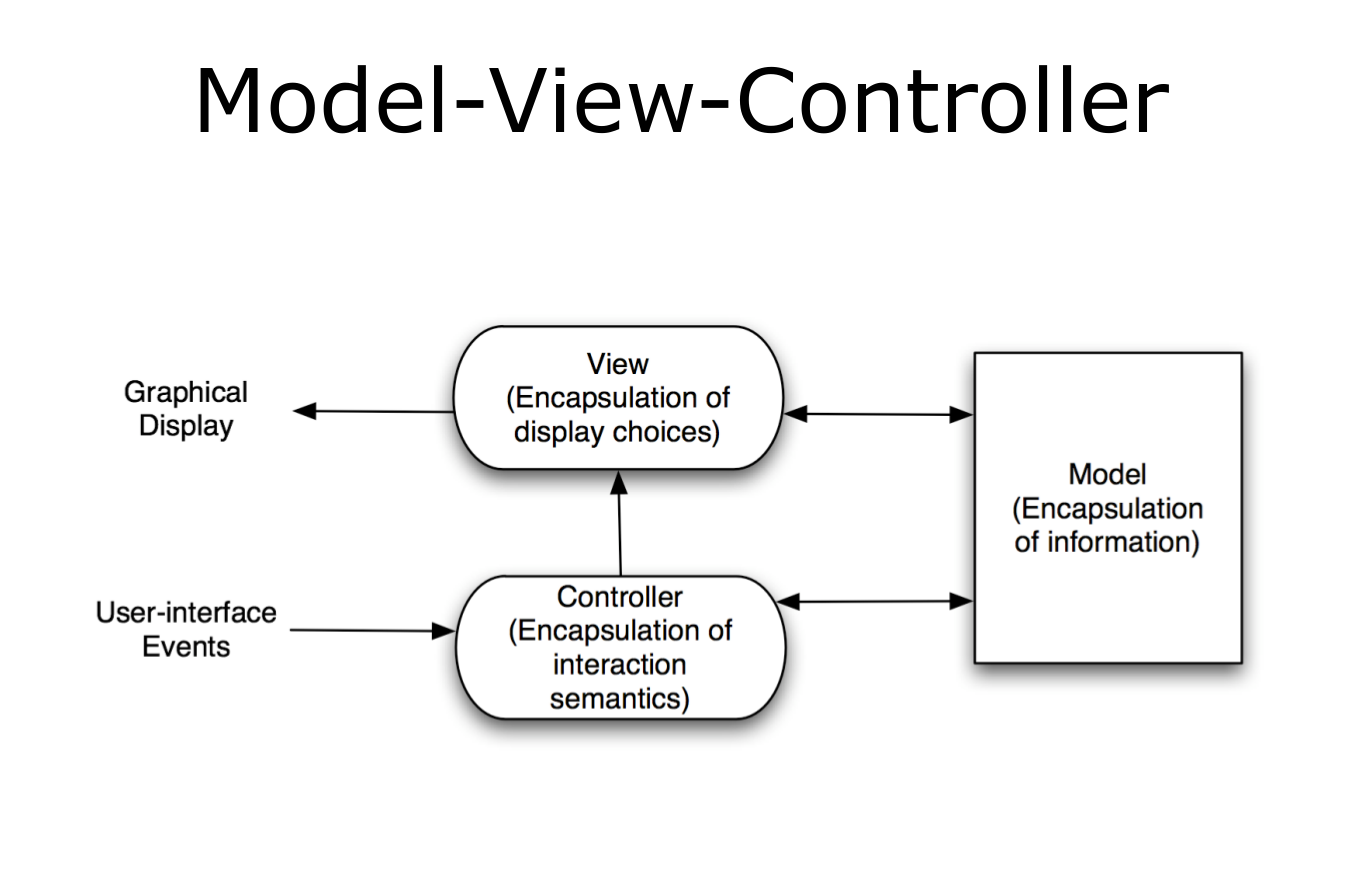
\includegraphics[width=1.2\linewidth]
  {images/3-model-view-controller.png}
\end{subfigure}
%\caption{-}
\end{figure}


% IMAGE:
\begin{figure}[H]
\hskip-2.5cm\begin{subfigure}{1.2\textwidth}
  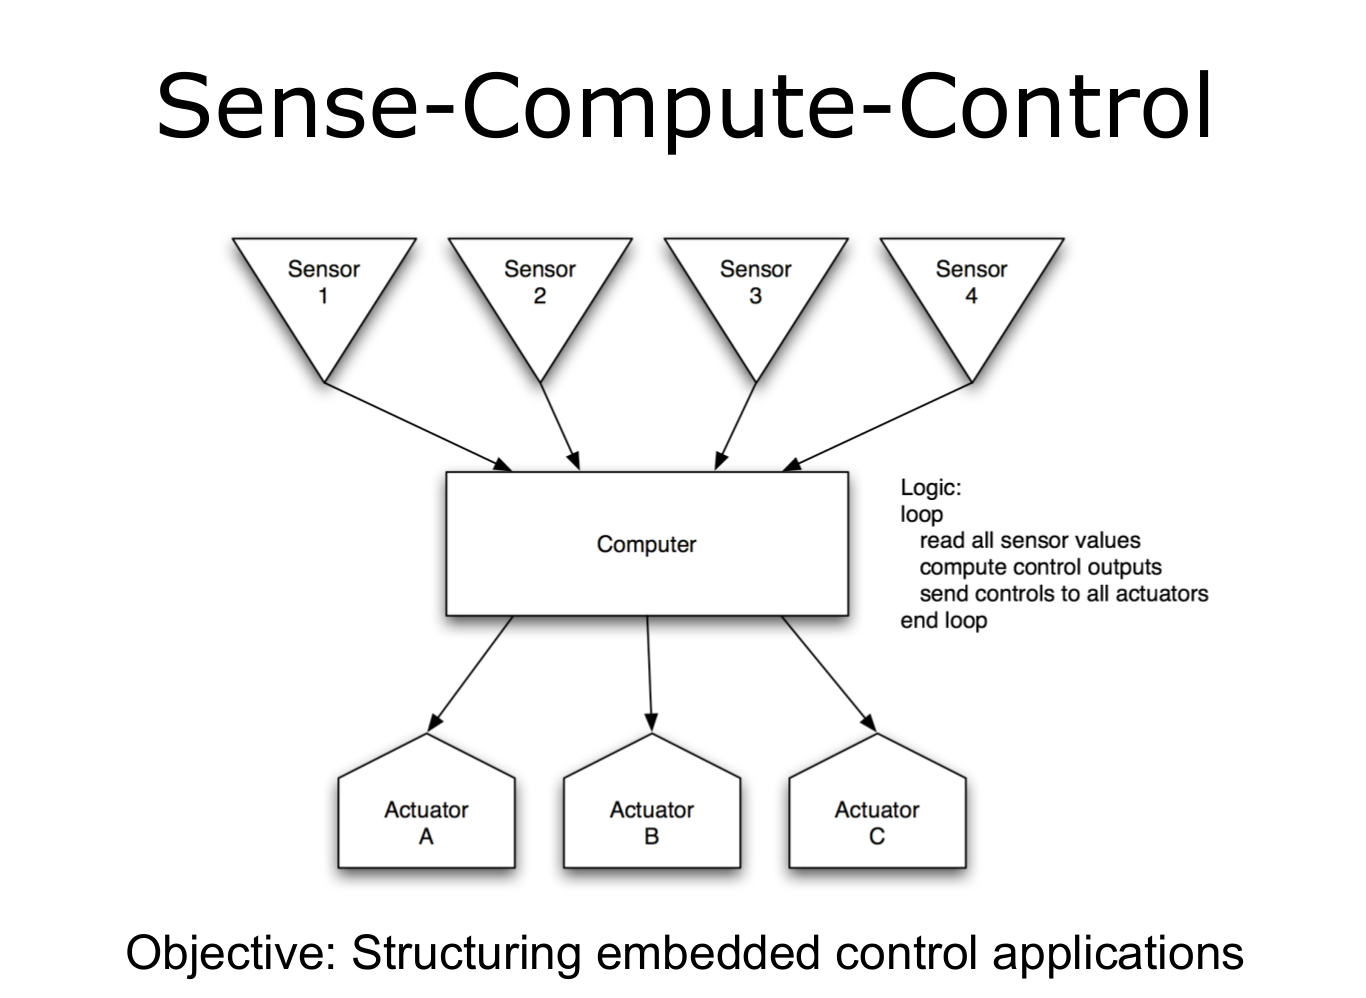
\includegraphics[width=1.2\linewidth]
  {images/3-sense-compute-control.png}
\end{subfigure}
%\caption{-}
\end{figure}

\section{Quality Attributes}

\section{QA: Availability}

\section{QA: Performance}

\section{QA: Security}

\section{QA: Testability}

\section{QA: Modifiability}

\newpage
\section{Connectors}

\textbf{Software connectors} are key elements of the software's architecture. They define the rules of \textbf{interaction} between \textbf{components}. There are various levels of software connectors that range from \textit{simple} to \textit{complex} connections.
\begin{itemize}
\item Simple: shared variable access, method calls ...
\item Complex: database access, client-server, scheduler, load balancer ...\\
\end{itemize}

In a projects \textbf{code base} the connections between components are often implicit and can be noticed easily. In the architecture design we \textbf{explicitly identify} them, to allow us to capture \textbf{system interactions} (at the level of the components). The specification for interactions are often \textit{complex.} An example for \textbf{LinkedIn} is provided below:\\

% IMAGE: LinkedIn Data
\begin{figure}[H]
\centering
\hskip-2.5cm\begin{subfigure}{1\textwidth}
  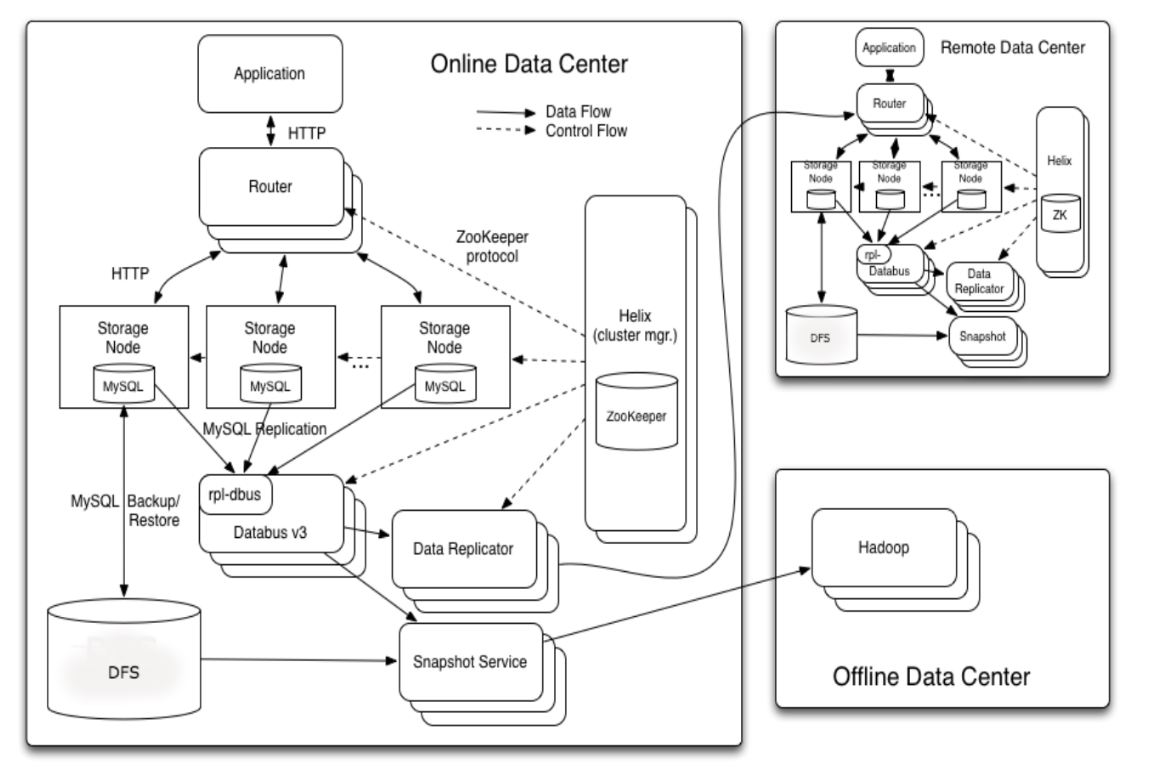
\includegraphics[width=1\linewidth]
  {images/10-linked.png}
\end{subfigure}
%\caption{-}
\end{figure}

% IMAGE: LinkedIn Redliner
\begin{figure}[H]
\centering
\hskip-2.5cm\begin{subfigure}{1\textwidth}
  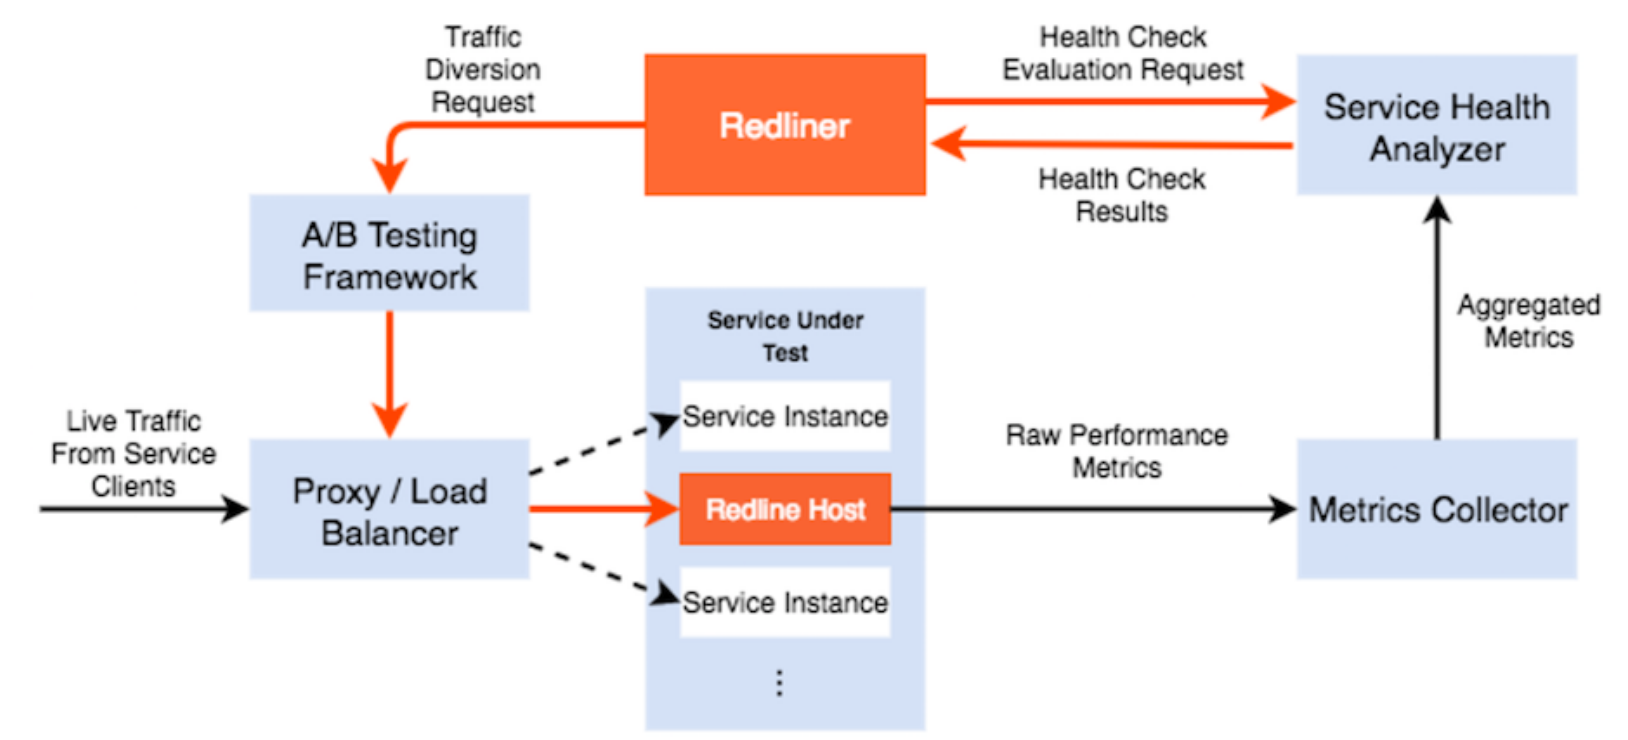
\includegraphics[width=1\linewidth]
  {images/10-linked-redliner.png}
\end{subfigure}
%\caption{-}
\end{figure}

\subsection{What is Different About Connectors?}
Depending on the software project, \textbf{components} will have \textbf{application-specific} functionality. \textbf{Connectors} provide \textit{interaction mechanisms} that are \textit{generic} across different application. \textbf{Interaction} may involve \textbf{multiple components}, and may have a protocol associated to it.\\

\subsection{Benefits of Explicit Connectors}
\begin{itemize}
\item \textbf{Interaction} is defined by the arrangement of the connectors (as far as possible)
\item \textbf{Component interaction} is defined by the pattern of connectors in the architecture
\item \textbf{Interaction} is \textit{"independent"} of the components
\end{itemize}

\subsection{Roles Played By Software Connectors}
The specification of the connector protocols determine:
\begin{itemize}
\item The types of interfaces
\item Properties of interaction
\item Riles about ordering interaction
\item Measurable features of interactions\\
\end{itemize}

Connectors often have multiple roles, the main roles are:
\begin{itemize}
\item Communication
\item Coordination
\item Conversion
\item Facilitation
\end{itemize}

\subsection{Communication}
Information is transmitted between \textbf{components} (e.g. message passing; method calls). \textbf{Connectors} constrain:
\begin{itemize}
\item \textbf{Direction of flow }(The pipes in the image below)
\item \textbf{Capacity / rate of flow}\\
\end{itemize}

** Additional Information **
\begin{itemize}
\item Connector providing communication services support \textbf{transmission} of data among components
\item Data transfer services are a primary building block of component interaction
\item Components routinely pass messages, exchange data to be processed and communication results of computations
\end{itemize}

% IMAGE: Pipes
\begin{figure}[H]
\centering
\hskip-2.5cm\begin{subfigure}{1\textwidth}
  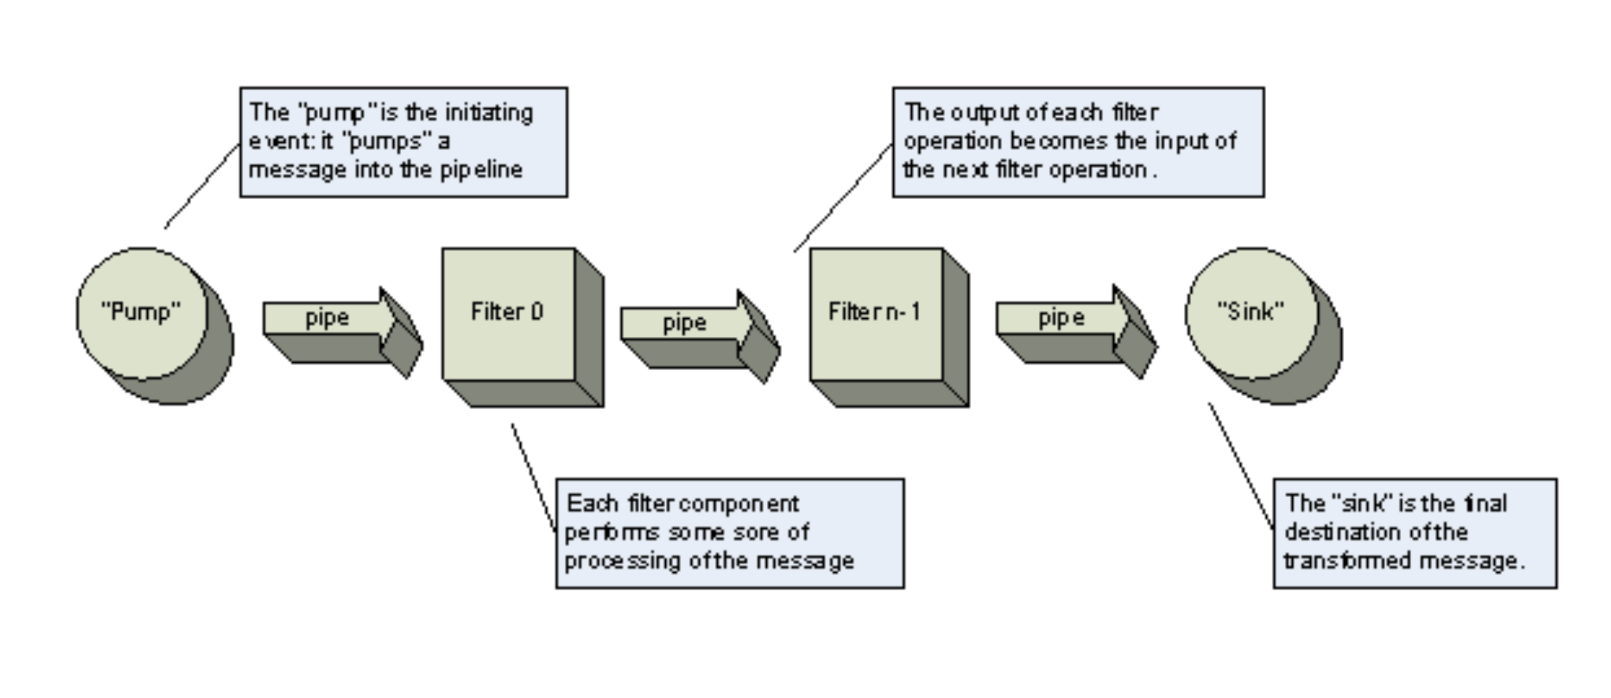
\includegraphics[width=1\linewidth]
  {images/10-pipes.png}
\end{subfigure}
%\caption{-}
\end{figure}

Connectors influence measurable quality attributes of the system. It separates \textbf{communication} from functional aspects.
\subsection{Coordination}
\textbf{Coordination} controls the timing \textbf{relationship} of the functional aspects of the system. \\

** Additional Information ** 
\begin{itemize}
\item Connectors providing coordination services support transfer of \textbf{control} among components
\item Components interact by passing the thread of execution to each other
\item \textbf{Function calls and method invocations are examples of coordination connectors}
\item Higher-order connectors, such as signals and load balancing connectors provide richer, more complex interaction built and coordination services
\end{itemize}

\subsection{Conversion}
\textbf{Conversion} is how to get components to interact that \textbf{do not} have the right means of interaction. \textbf{Incompatibilities} might be related to: datatypes, ordering, frequency, structure of parameters etc ...\\

Examples of types of converters:
\begin{itemize}
\item Wrappers: deal with structural issues
\item Adaptors: deal with datatype incompatibilities\\
\end{itemize}

** Additional Information **
\begin{itemize}
\item Connectors providing conversion services \textbf{transform the interaction} required by one component to that provided by another
\item Enabling heterogeneous components to interact with each other is \textbf{not} a trivial task
\item Conversion services allow components that have not been specifically tailored for each other to establish and conduct interaction
\end{itemize}

\subsection{Facilitation}
\textbf{Facilitation} enables interaction among a group of components that are intended to interact with one and other.

** Additional Information ** 
\begin{itemize}
\item Improve interaction of components that were intended to interoperate (usually \textbf{optimise} or streamlines interactions)
\item Ensure proper performance profiles (load balancing or scheduling)
\item Synchronization mechanisms (monitors $\rightarrow$ enforce mutex access to resources)
\end{itemize}

\subsection{Types of Connectors (Talyor, Medvidovic \& Dashofy)}
\begin{table}[H]
\begin{tabular}{|l|p{10cm}|}
\hline
Connector & Description\\
\hline
Method/Procedure Call & Producre call connectors model the flow of control among components through various invocation techniques. They are thus \textbf{coordination connector}. [Examples: fork and exec]\\
\hline
Data Access & Data access connectors allow components to access maintained by a data store component. Therefore they provide \textbf{communication services}. [Example: JDBC $\rightarrow$ java SQL driver]\\
\hline
Event & An even as the instantaneous effect of the termination of the invocation of an operation on an object, which occurs at that object's location. [Example: windows with GUI inputs] \\
\hline
Stream & Streams are used to preform transfer of large amounts of data between autonomous processes. Thus they provide \textbf{communication services} in a system. [Examples: UNIX pipes, TCP/UDP sockets, client-server protocols]\\
\hline
Distributor & Distributor connectors perform the identification of interaction paths and subsequent routing of communication and coordination information among components along these paths. They provide \textbf{facilitation} services. \textit{[Distributor connectos never exist by themselves, but provide assistance to other connectors, such as steams or procedure calls)}\\
\hline
Arbitrator & When components are aware of the presence of other components but cannot make assumptions about their needs and state, arbitrators streamline system operation and resolve any conflicts (providing \textbf{facilitation}). They also redirect the flow of control (providing \textbf{coordination}) \\
\hline
Adaptor & Adaptor connectors provide facilities to support interaction between components that have not been designed to interoperate. \textit{(adopters involve matching communication polices and interaction protocols among components, thus providing \textbf{conversion} services.}\\
\hline
\end{tabular}
\end{table}

\section{Patterns}

\section{Modelling The Life-cycle}

\section{Dev-Ops}

\section{Product Line Architecture}

\section{Analysis}








\end{document}
